\chapter{Androidアプリ「LEDOXEA」}
\label{chap:ledoxea}

本章では、開発したAndroidアプリ「LEDOXEA」の利用方法と、その特徴について説明する。

\section{使用方法}
起動後、図\ref{le01}のような画面が表示される。上部にある検索ボックスをタップすると図\ref{le02}のようにソフトキーボードが表示されるので、ここに検索したいキーワードを入力する。日本語入力も可能である。入力が完了したら、図\ref{le03}のように右側の検索ボタンを押下する。すると検索が行われ、図\ref{le04}のように、合計5本のラインと星形のコンテンツ一覧が画面上に出現する。これらを上下にスワイプすると、図\ref{le05}のように、検索結果を上下に移動できる。これにより、ひとつひとつ項目を参照することが可能である。また、別の種類のコンテンツを参照したい時は左右にスワイプする。すると、図\ref{le06}のように、回転ハンガーのようにコンテンツが隣のコンテンツまで回転し、別のコンテンツが中央に移動し、上下のスワイプで同様に閲覧が可能となる。詳しく見たいコンテンツがある場合、画面下部に表示されたタイトル・サマリーの表示部分をタップすると外部アプリやブラウザが起動し、コンテンツの閲覧に即座に移動する。見終わった後、デバイス上のバックボタンを押すとグラフの画面に戻り、別の結果の確認へと移ることができる。

\begin{figure}[htbp]
 \begin{minipage}{0.45\hsize}
  \begin{center}
   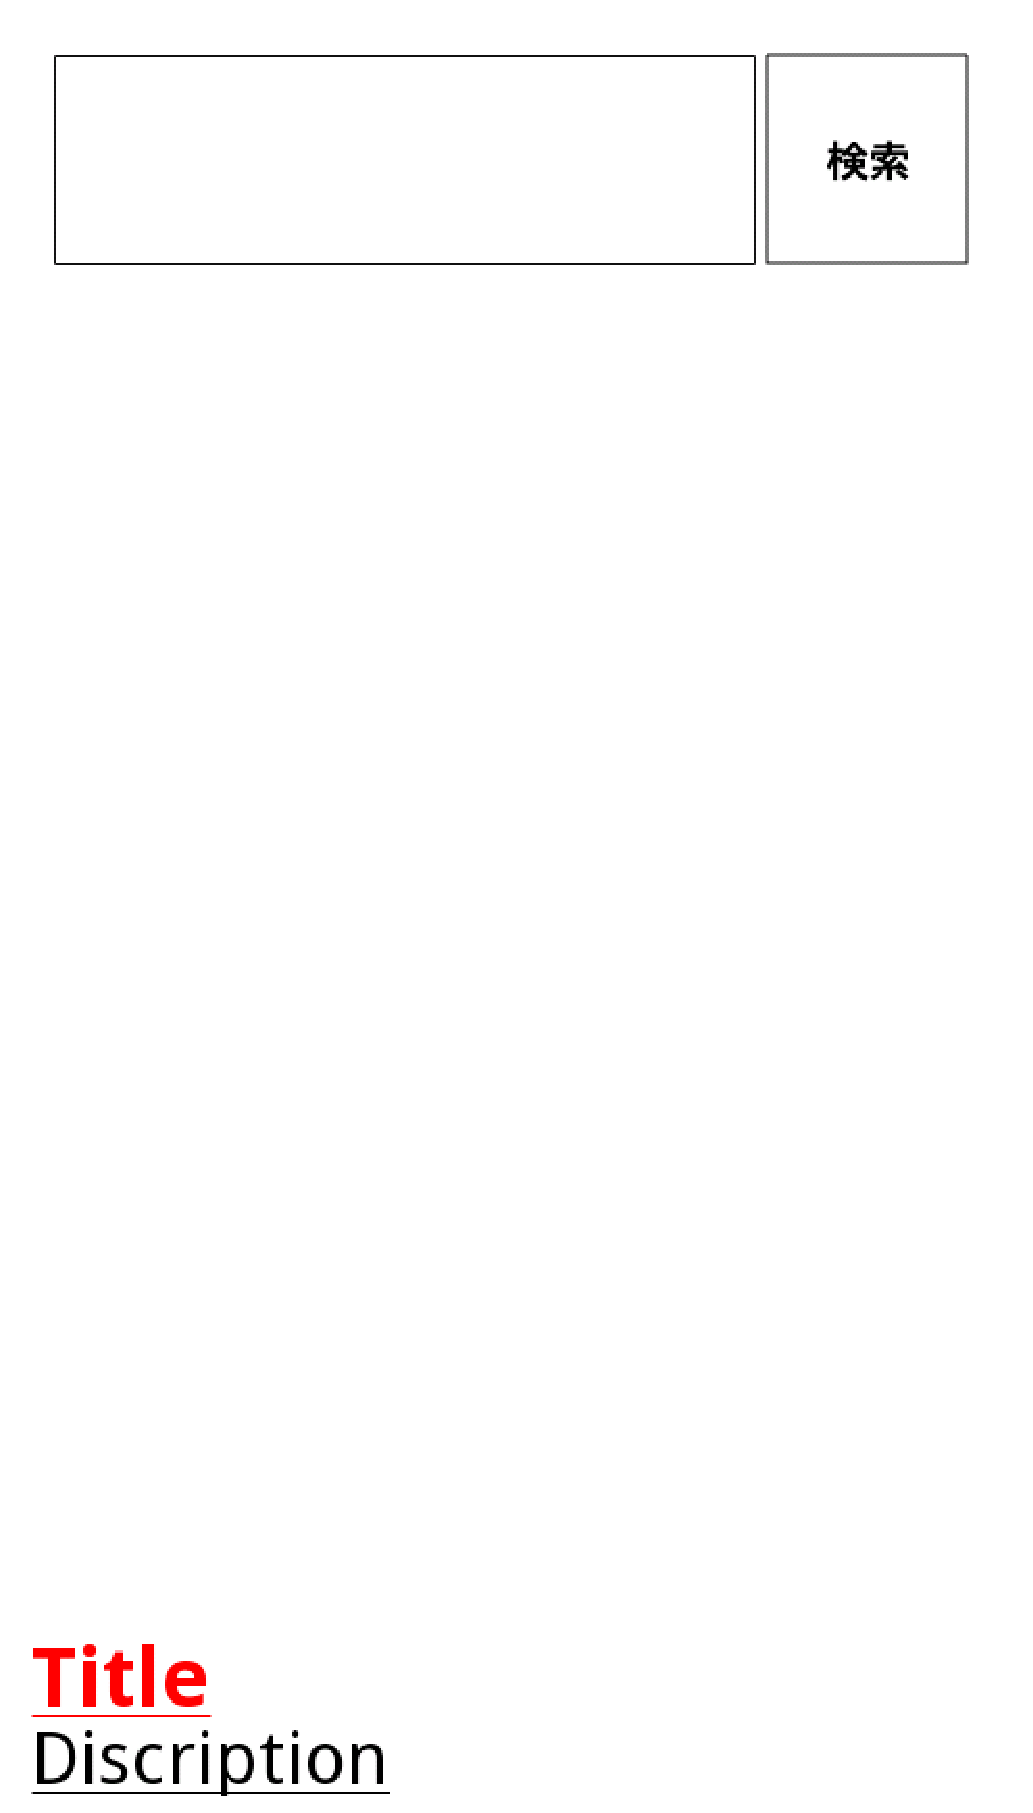
\includegraphics[height=90mm]{eps/le01.eps}
  \end{center}
  \caption{起動画面}
  \label{le01}
 \end{minipage}
 \begin{minipage}{0.45\hsize}
  \begin{center}
   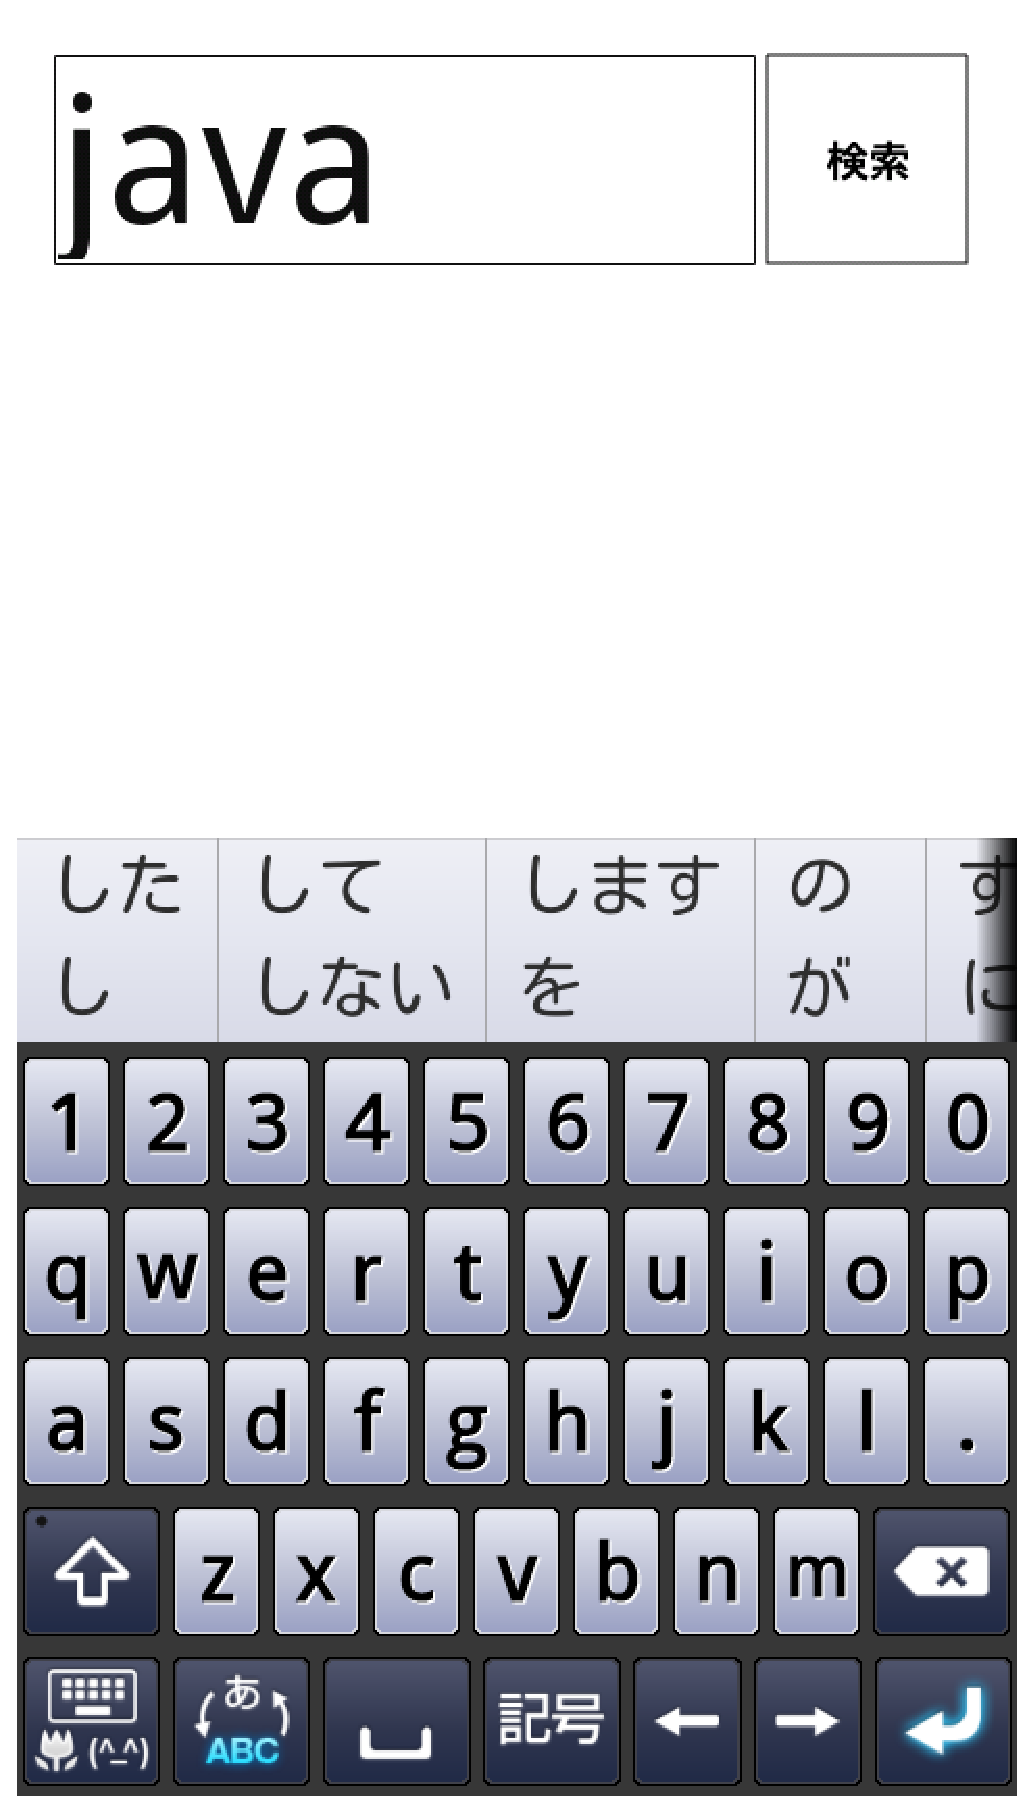
\includegraphics[height=90mm]{eps/le02.eps}
  \end{center}
  \caption{検索キーワードを入力}
  \label{le02}
 \end{minipage}
\end{figure}

\begin{figure}[htbp]
 \begin{minipage}{0.45\hsize}
  \begin{center}
   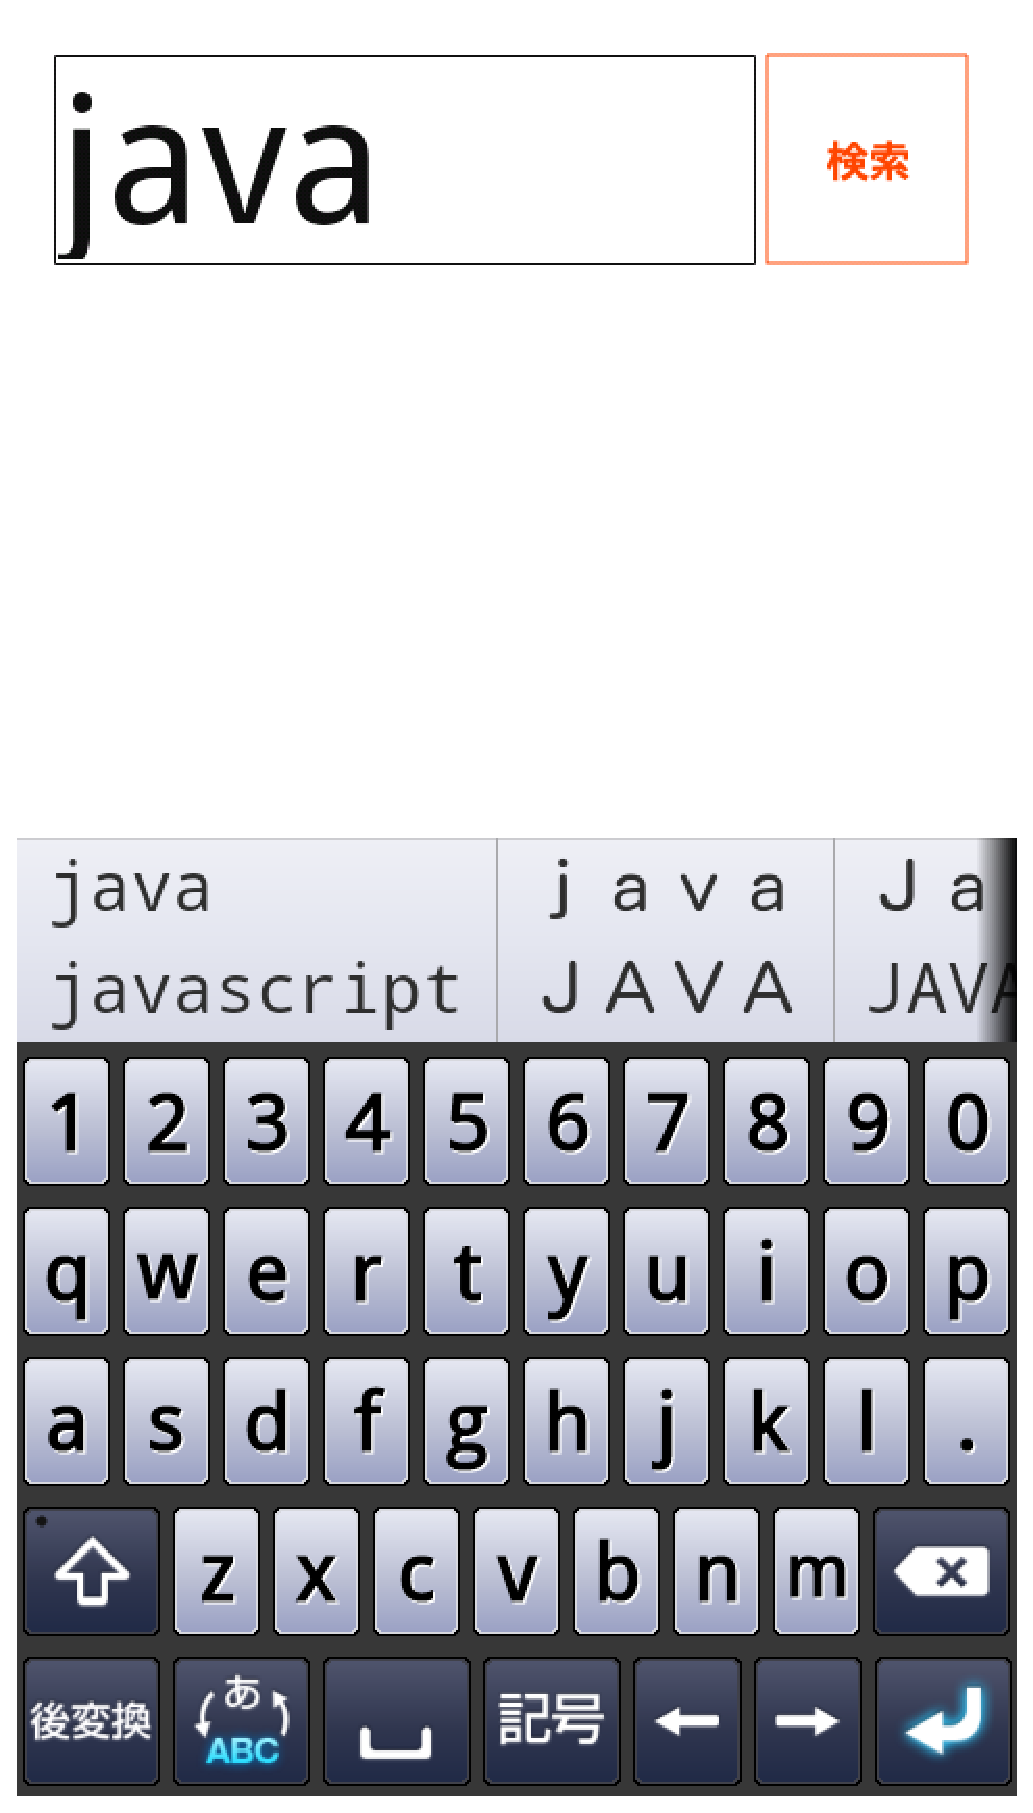
\includegraphics[height=90mm]{eps/le03.eps}
  \end{center}
  \caption{検索ボタンを押下}
  \label{le03}
 \end{minipage}
 \begin{minipage}{0.45\hsize}
  \begin{center}
   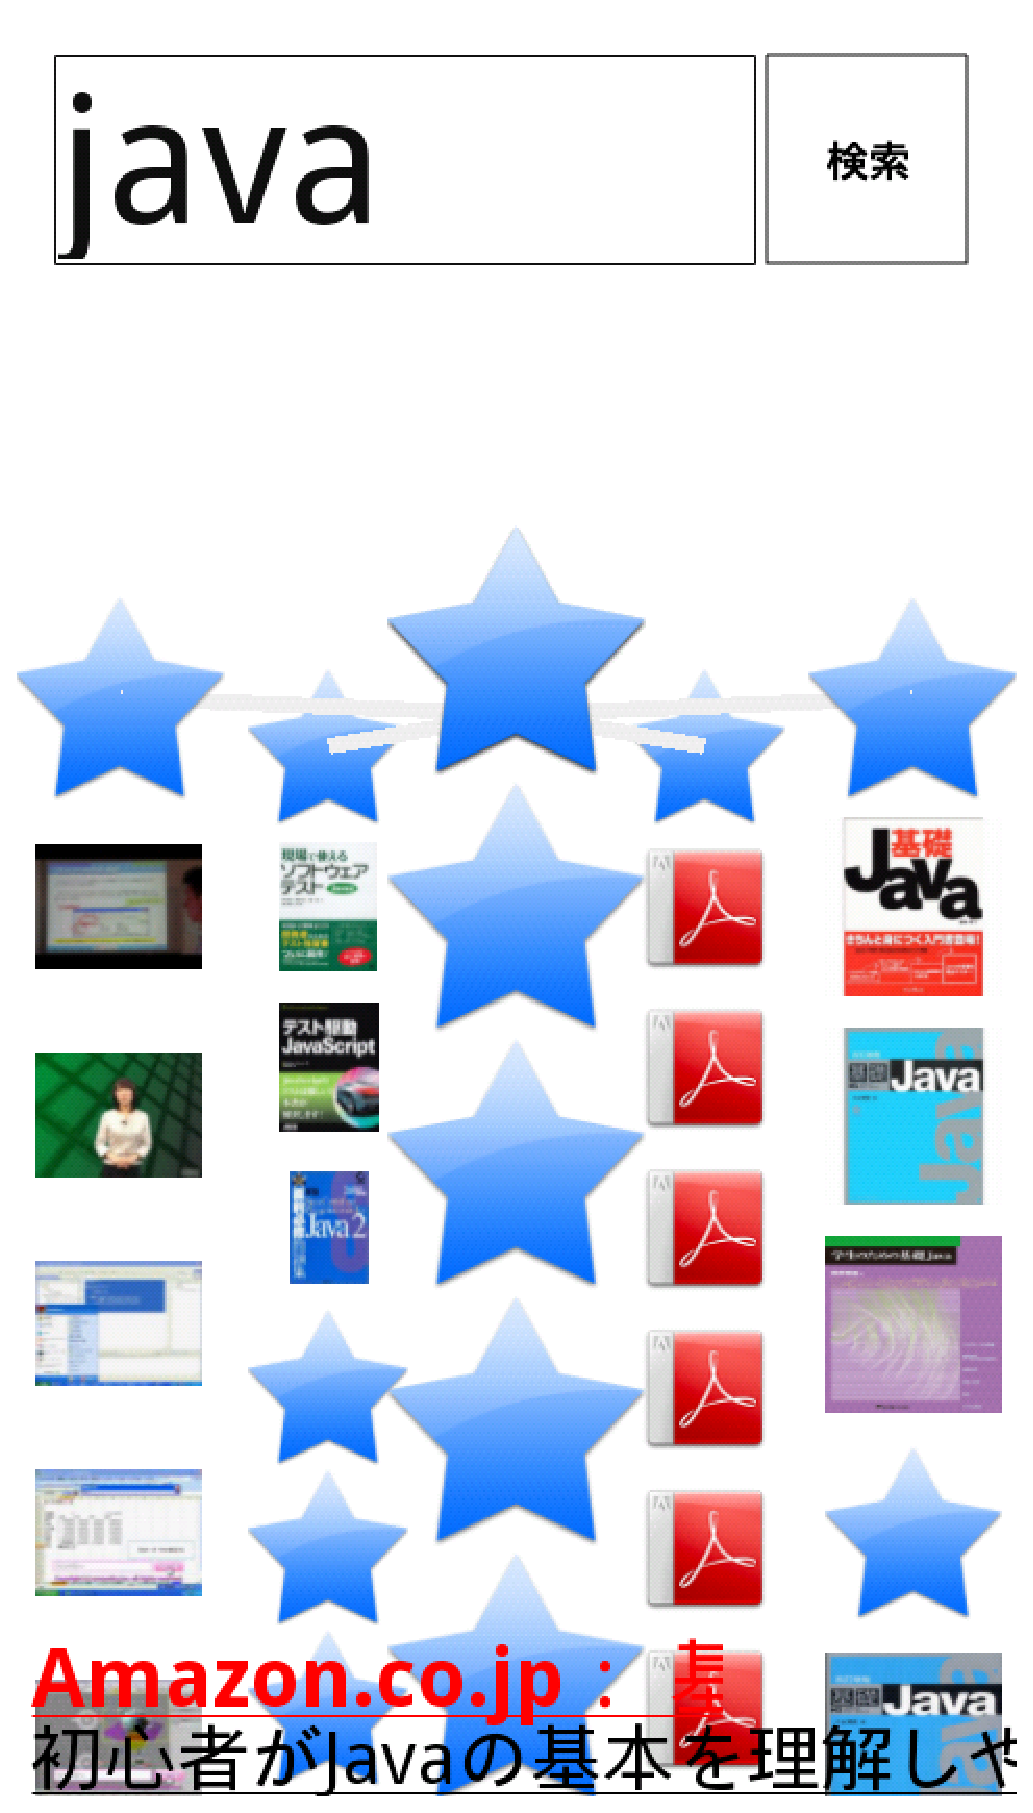
\includegraphics[height=90mm]{eps/le04.eps}
  \end{center}
  \caption{コンテンツ表示}
  \label{le04}
 \end{minipage}
\end{figure}

\begin{figure}[htbp]
 \begin{minipage}{0.45\hsize}
  \begin{center}
   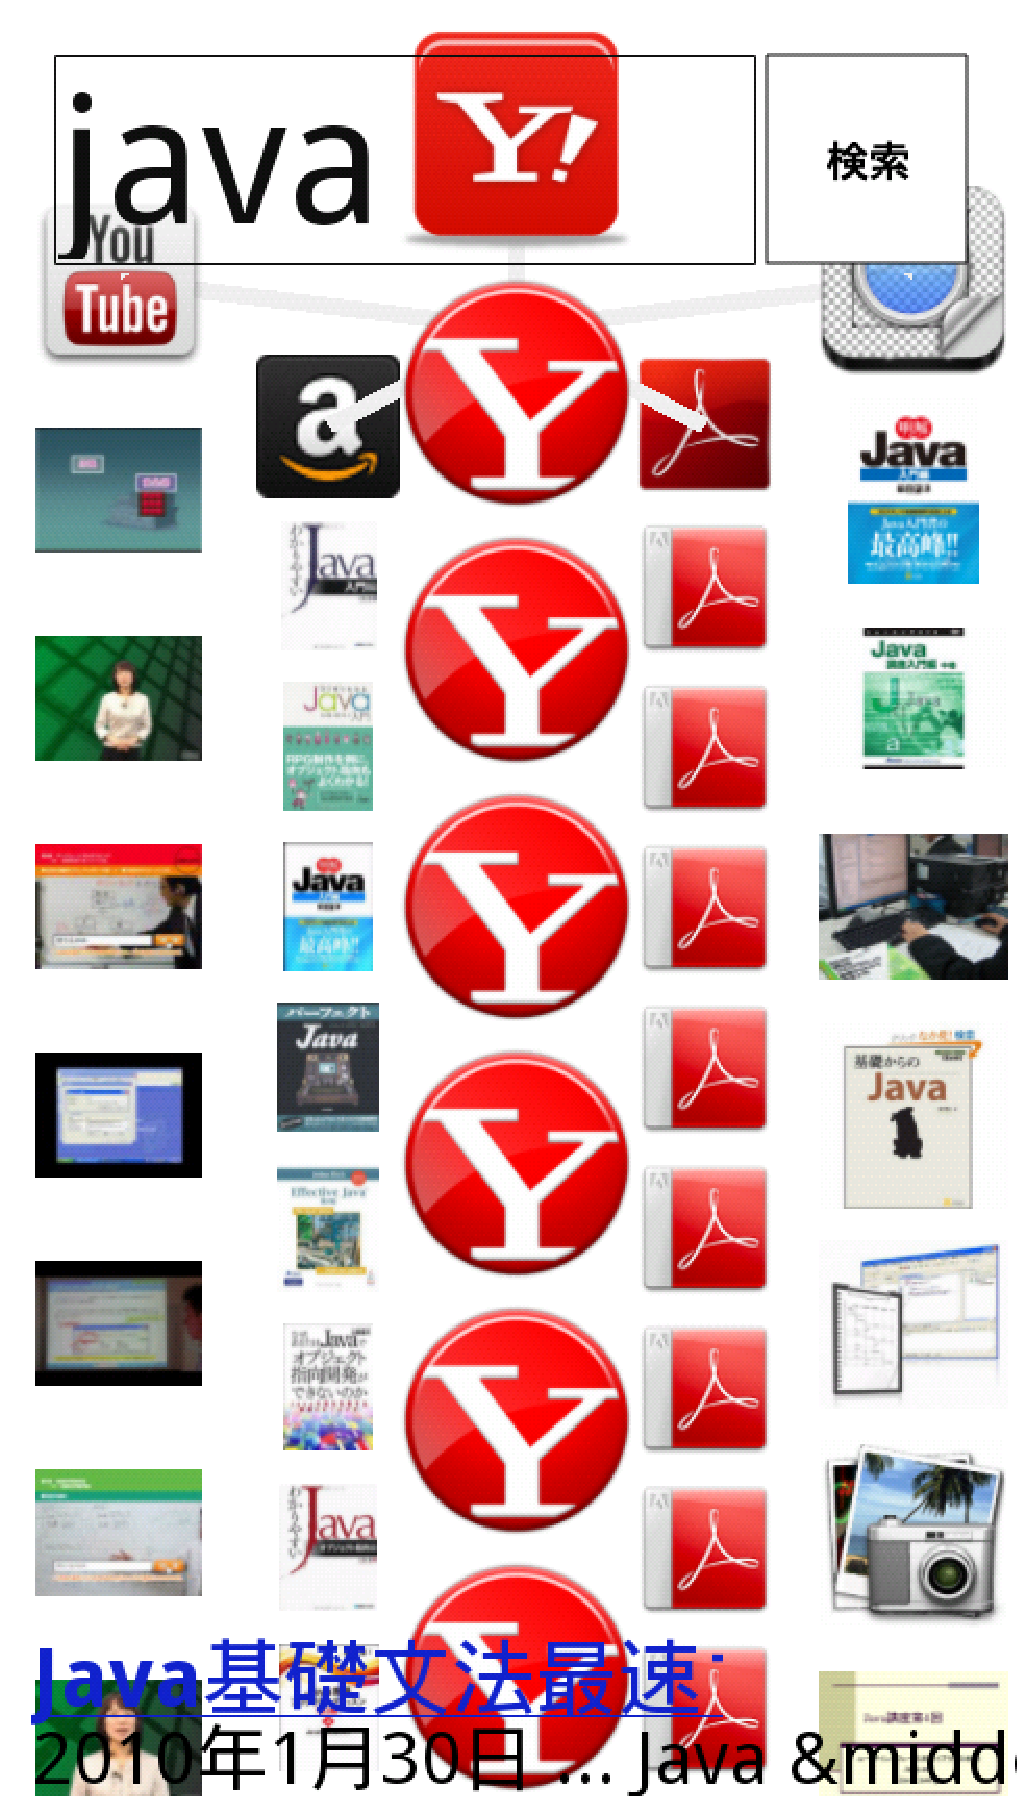
\includegraphics[height=90mm]{eps/le05.eps}
  \end{center}
  \caption{上にスワイプで上下移動}
  \label{le05}
 \end{minipage}
 \begin{minipage}{0.45\hsize}
  \begin{center}
   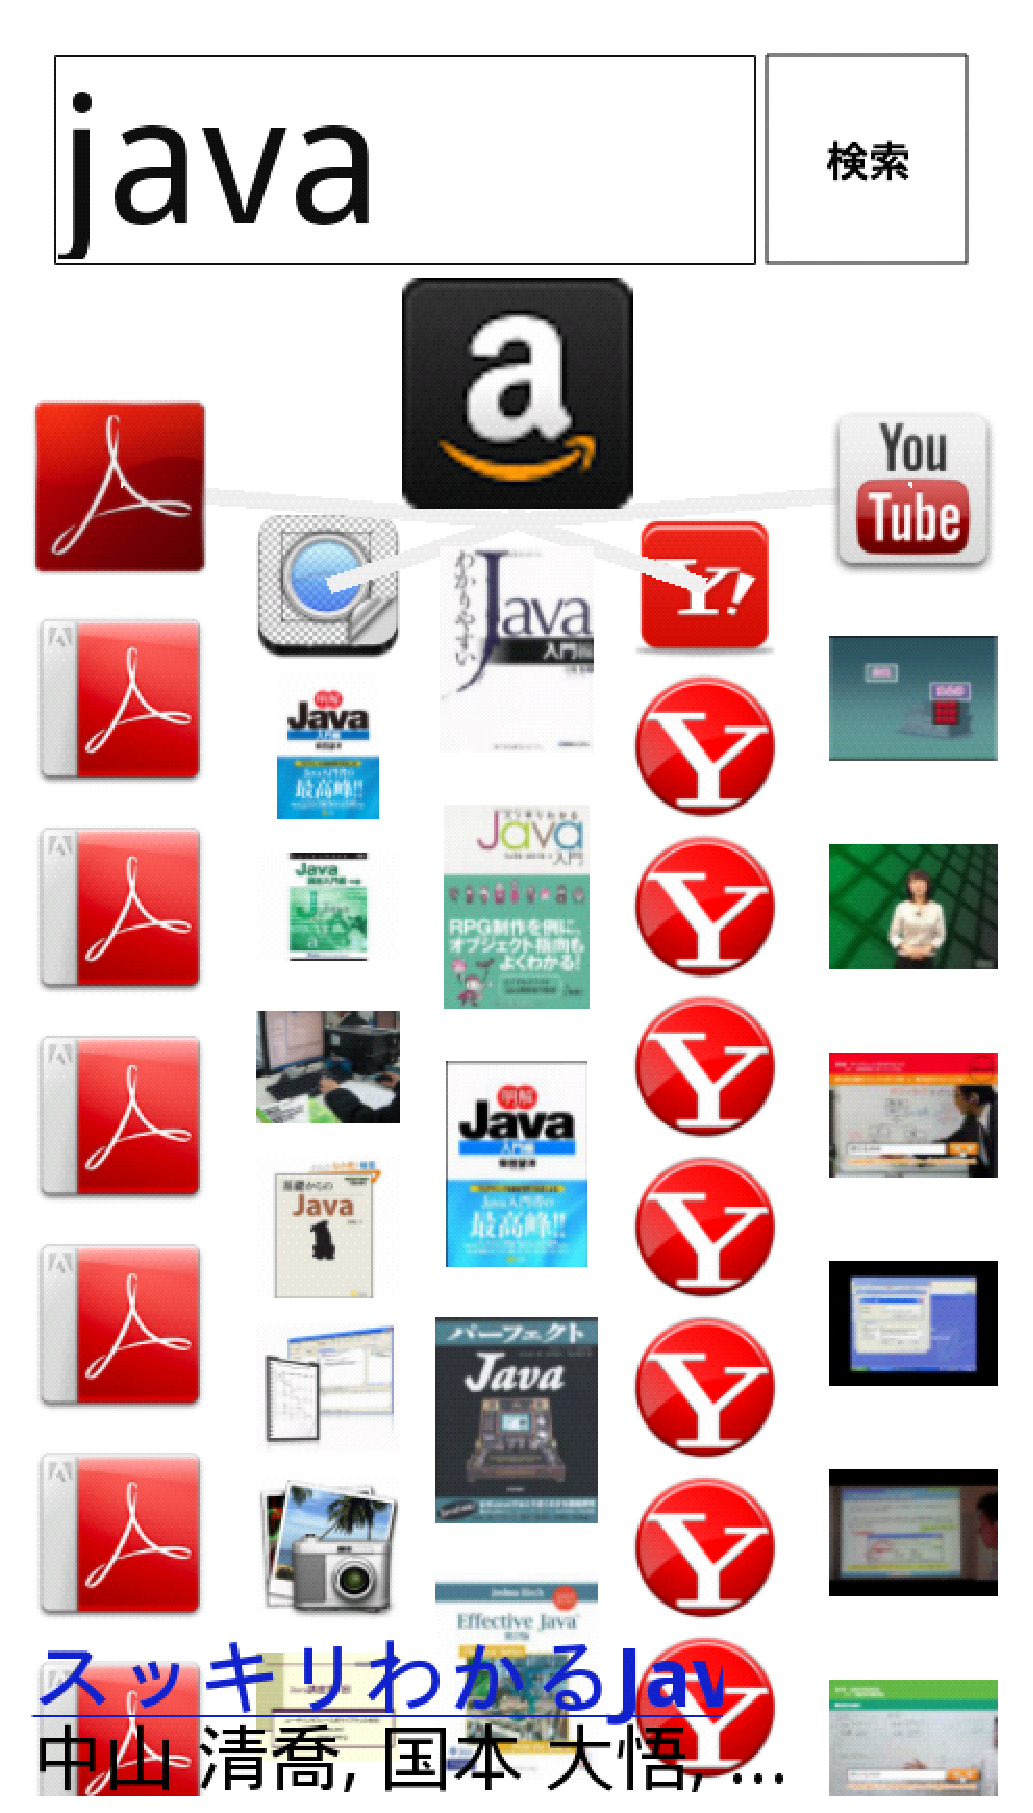
\includegraphics[height=90mm]{eps/le06.eps}
  \end{center}
  \caption{横にスワイプで}
  \label{le06}
 \end{minipage}
\end{figure}

\section{特徴}
それぞれ実現することができた、特徴について記述する。

\subsection{移植性}
ADOBE AIR の移植性の高さにより、Androidに留まらず、iOS、PCのWebブラウザ、PCアプリケーションとして、将来的に様々な形態、画面サイズに対応できる。

\subsection{スペック性能への非依存性}
非常に簡易な3次元CGにより製作されているため、30fps程度の安定した高速描画を実現している。コンテンツ間の移動にもカメラが線形に移動することで、滑らかに移動過程がレンダリングされるようになっている。

\subsection{フリック操作、画像ノードによる直感的操作性}
検索結果を上下や左右に移動することは、指先を使った移動方法として直感的に理解しやすく、項目を確認する際に発生する苦痛を軽減することが可能になる。また、グラフ表示上のノードに画像を採用したことにより、より内容が分かりやすく理解可能となった。

\subsection{検索エンジンの同時検索、WWW視覚化}
e-learningコンテンツを複数の検索エンジンで同時に高精度で検索できるため、一度の検索で非常に多くの有用な検索結果を得ることができる。